%\chapter{Desenvolvimento}

\chapter{Estudo de Caso}

Com o escopo do projeto definido e os conceitos apresentados, podemos apresentar o resultado da implementação. Os testes foram executados para os quatro circuitos descritos: O filtro passa-banda Sallen-Key, o filtro universal (CTSV – Continuous Time State-variable), o filtro passa-alta ativo Biquad (BIQUAD – our Opamp Biquad Highpass Filter) e Retificador não-linear. Os procedimentos para a realização das avaliações são aqueles explicados no capítulo 4, os quais necessitam da obtenção dos conjuntos de treinamento e teste.

Os conjuntos de treinamento e teste são obtidos em duas etapas diferentes. Primeiro, o circuito a ser avaliado é modelado na plataforma de simulação do LTSpice para simulação e modelagem de circuitos eletrônicos.   Sabendo que cada classe de falha apresenta 300 dados contínuos (parâmetro definido) podemos variar o valor do parâmetro (componente) da classe correspondente a cada 300 dados.  Assim um número total de classes de cada circuito de �� = ��300 classes, sendo K a quantidade de falhas pré definidas, falhas no caso é qualquer alteração acima ou abaixo da faixa de tolerância nos componentes do circuito. 

\begin{table}[ht]
\centering
\begin{tabular}{ccc}
\textbf{Circuito}      & \textbf{Nº Falhas} & \textbf{Nº Dados} \\
Filtro Biquadrado      & 12                 & 3900              \\
CSTV                   & 18                 & 6000              \\
Retificador Não linear & 10                 & 3300              \\
Sallen Key             & 10                 & 3300             
\end{tabular}
\caption{\label{tab:resultado}- Falhas dos circuitos}
\end{table}


Na segunda etapa é realizada a transferência dos dados obtidos nas simulações do LTSpice para a leitura em python. Além da dificuldade inicial de realizar a leitura dos dados devido ao modo de construção do arquivo '.raw', foi necessário fazer uma série de validações e manipulações de dados para os deixar em formato pronto para processar.Além disso existia muita informação desnecessária, como a predição aconteceria em relação a Vout, não existe a necessidade de armazenar e manter os dados de medição dos demais nós e componentes do circuito. Esse processo reduziu o volume de dados drasticamente. Após esse processo, os dados são duplicados para termos o conjunto de treino e teste separados.
Uma informação importante a ser destacada são os atributos dos classificadores implementados: DecisionTreeClassifier(random\_state=20);  AdaBoostClassifier(random\_state=20); svm.SVC(kernel='linear', C=1,
random\_state=20); RandomForestClassifier(random\_state=20); GaussianNB(); KNeighborsClassifier(); SGDClassifier(random\_state=20); LogisticRegression(random\_state=20)


\section{\textbf{Sallen Key}}

Usando os códigos que estão anexados no apêndice  foi realizada a aquisição dos dados e tratamento inicial.

 Nas imagens a seguir temos o gráfico do estágio inicial. A  \ref{fig:dadoSalleninicial} exibe os recém adquiridos, mas já manipulado e limpo, ou seja, após o tratamento inicial. 
        
 \begin{figure}[H]
        \begin{center}
        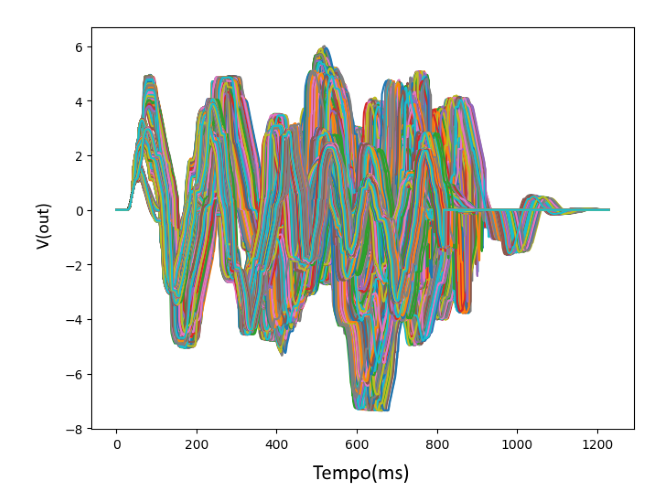
\includegraphics[width=15cm]{./01_Pre_textuais/sallen_figs/dadosPreProc_Sallen_Key_mc_+_4bitPRBS_[FALHA]raw.png}
        \caption{\label{fig:dadoSalleninicial}- Circuito: Sallen key - Dados iniciais (Vout x Time).}
        \end{center}
        \end{figure}
        
Após a aplicação de PAA e PCA temos um conjunto de dados com apenas 5\% dos dados originais. A \ref{fig:pcaSalenkey} exibe os dados limpos e antes de entrar no classificador.

 \begin{figure}[H]
        \begin{center}
        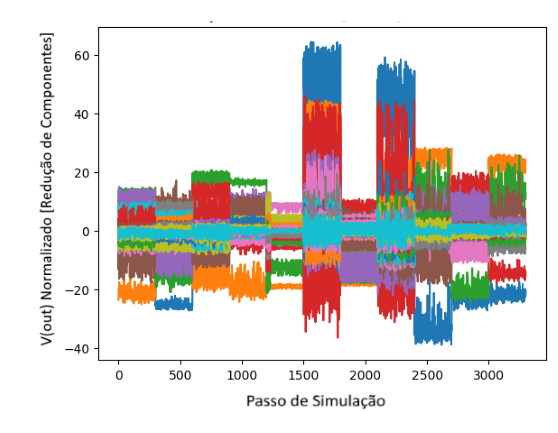
\includegraphics[width=13cm]{./05_Cap5/figures/PCA_Sallen_Key_mc_+_4bitPRBS_[FALHA]raw.png}
        \caption{\label{fig:pcaSalenkey}- Circuito: Sallen key - Dados após processamento (Vout x Time)}
        \end{center}
        \end{figure}

O sistema é classificado com oito métodos diferentes descritos anteriormente e com as falhas determinadas na \ref{tab:falhasckt1}. 

A seguir descrevemos a taxa de acerto para cada um dos algoritmos. 


 
\begin{itemize}
\newpage
 \item Classificador por Árvore de decisão
 
\begin{table}[ht]
\centering
\begin{tabular}{ccc}
\textbf{Classe} & \textbf{Acerto (\%)} & \textbf{Acurácia (\%)} \\
Classe 1        & 100                  & 100                    \\
Classe 2        & 0                  & 0                    \\
Classe 3        & 0                  & 0                    \\
Classe 4        & 0                  & 0                    \\
Classe 5        & 0                  & 0                    \\
Classe 6        & 0                  & 0                    \\
Classe 7        & 0                  & 0                    \\
Classe 8        & 0                  & 0                    \\
Classe 9        & 0                  & 0                    \\
Classe 10       & 0                  & 0                    \\
Classe 11       & 0                  & 0                                       
\end{tabular}
\caption{\label{tab:sallenarvore}- Sallen Key: Falhas Árvore de decisão}
\end{table}

 \begin{figure}[H]
        \begin{center}
       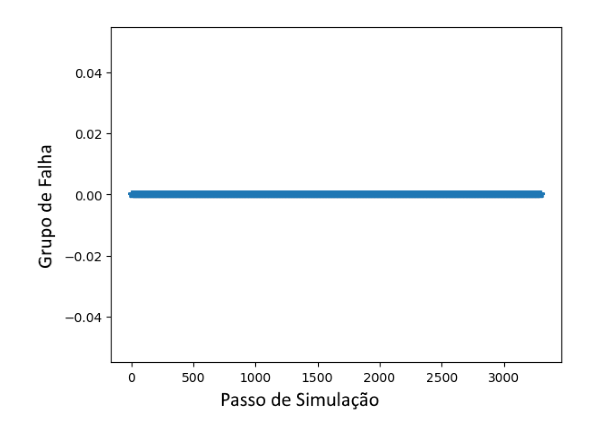
\includegraphics[width=13cm]{./01_Pre_textuais/sallen_figs/DecisionTreeClassifier_Sallen_Key_mc_+_4bitPRBS_[FALHA]raw.png}
        \caption{\label{fig:DecisionTreeClassifieSalenkey}- Circuito: Sallen key - Comportamento da Predição Árvore de decisão}
        \end{center}
        \end{figure}
        
        

A percentual de acerto total é de 9\% para o circuito Sallen Key exemplificado na \ref{fig:DecisionTreeClassifieSalenkey} e \ref{tab:sallenarvore}. 
\newpage
 \item Classificador AdaBoost
 
 \begin{table}[ht]
\centering
\begin{tabular}{ccc}
\textbf{Classe} & \textbf{Acerto (\%)} & \textbf{Acurácia (\%)} \\
Classe 1        & 100                  & 100                    \\
Classe 2        & 100                  & 100                    \\
Classe 3        & 99                  & 99.5                    \\
Classe 4        & 100                  & 100                    \\
Classe 5        & 100                  & 100                    \\
Classe 6        & 100                  & 100                    \\
Classe 7        & 100                  & 100                    \\
Classe 8        & 100                  & 100                    \\
Classe 9        & 100                  & 100                    \\
Classe 10       & 100                  & 100                    \\
Classe 11       & 100                  & 100                               
\end{tabular}
\caption{\label{tab:sallenAdaBoost}- Sallen Key: Falhas AdaBoost}
\end{table}


 \begin{figure}[H]
        \begin{center}
        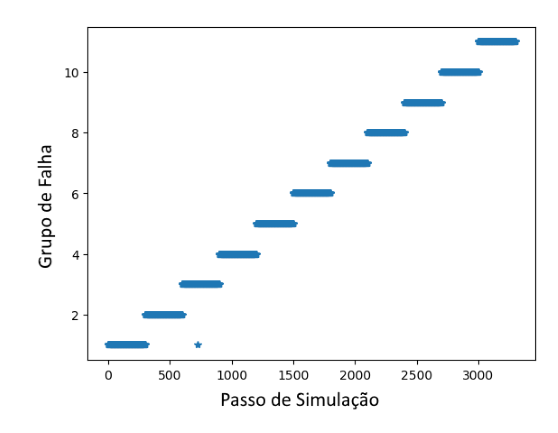
\includegraphics[width=13cm]{./01_Pre_textuais/sallen_figs/AdaBoostClassifier_Sallen_Key_mc_+_4bitPRBS_[FALHA]raw.png}
        \caption{\label{fig:AdaboostClassifieSalenkey}- Circuito: Sallen key - Comportamento da Predição Ada Boost }
        \end{center}
        \end{figure}
       

A percentual de acerto total é de 99,96\% para o circuito Sallen Key exemplificados na \ref{fig:AdaboostClassifieSalenkey} e \ref{tab:sallenAdaBoost}. 

\newpage
 \item Classificador Máquinas de vetores de suporte
 
 \begin{table}[ht]
\centering
\begin{tabular}{ccc}
\textbf{Classe} & \textbf{Acerto (\%)} & \textbf{Acurácia (\%)} \\
Classe 1        & 100                  & 100                    \\
Classe 2        & 0                  & 0                    \\
Classe 3        & 0                  & 0                    \\
Classe 4        & 0                  & 0                    \\
Classe 5        & 0                  & 0                    \\
Classe 6        & 0                  & 0                    \\
Classe 7        & 0                  & 0                    \\
Classe 8        & 98                  & 98                    \\
Classe 9        & 100                  & 100                    \\
Classe 10       & 100                  & 100                    \\
Classe 11       & 0                  & 0                               
\end{tabular}
\caption{\label{tab:sallensvm}- Sallen Key: Falhas SVC}
\end{table}

\begin{figure}[H]
        \begin{center}
        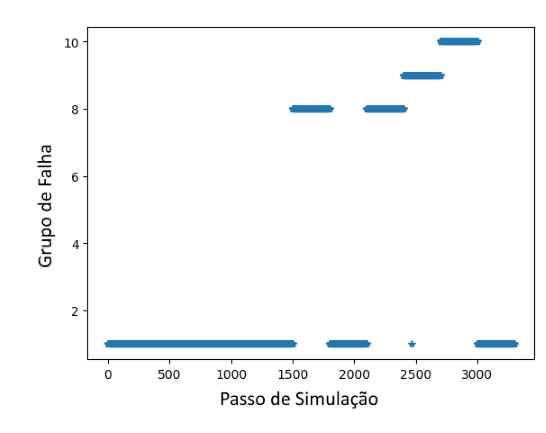
\includegraphics[width=13cm]{./01_Pre_textuais/sallen_figs/SVC_Sallen_Key_mc_+_4bitPRBS_[FALHA]raw.png}
        \caption{\label{fig:SVCClassifieSalenkey}- Circuito: Sallen key - Comportamento da Predição SVC}
        \end{center}
        \end{figure}
       

A percentual de acerto total é de 12,06\% para o circuito Sallen Key exemplificado na \ref{fig:SVCClassifieSalenkey} e \ref{tab:sallensvm}. 

\newpage

 \item Classificador Floresta aleatória
 
 \begin{table}[ht]
\centering
\begin{tabular}{ccc}
\textbf{Classe} & \textbf{Acerto (\%)} & \textbf{Acurácia (\%)} \\
Classe 1        & 100                  & 100                    \\
Classe 2        & 100                  & 100                    \\
Classe 3        & 100                  & 100                    \\
Classe 4        & 100                  & 100                    \\
Classe 5        & 100                  & 100                    \\
Classe 6        & 100                  & 100                    \\
Classe 7        & 100                  & 100                    \\
Classe 8        & 100                  & 100                    \\
Classe 9        & 100                  & 100                    \\
Classe 10       & 100                  & 100                    \\
Classe 11       & 100                  & 100                                  
\end{tabular}
\caption{\label{tab:sallenrandom}- Sallen Key: Falhas Floresta aleatória}
\end{table}


  \begin{figure}[H]
        \begin{center}
        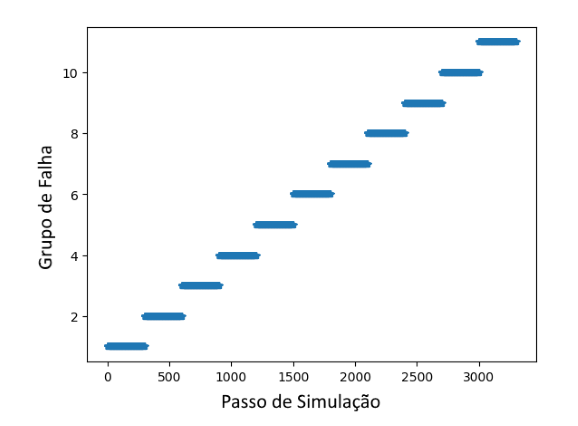
\includegraphics[width=13cm]{./01_Pre_textuais/sallen_figs/RandomForestClassifier_Sallen_Key_mc_+_4bitPRBS_[FALHA]raw.png}
        \caption{\label{fig:randomforestClassifieSalenkey}- Circuito: Sallen key - Comportamento da Predição Random Forest }
        \end{center}
        \end{figure}

A percentual de acerto total é de 100\% para o circuito Sallen Key exemplificado na \ref{fig:randomforestClassifieSalenkey} e \ref{tab:sallenrandom}. 

\newpage
 \item Classificador Gaussiano de Naive Bayes
 
 \begin{table}[ht]
\centering
\begin{tabular}{ccc}
\textbf{Classe} & \textbf{Acerto (\%)} & \textbf{Acurácia (\%)} \\
Classe 1        & 100                  & 100                    \\
Classe 2        & 100                  & 100                    \\
Classe 3        & 98                  & 99                    \\
Classe 4        & 100                  & 100                    \\
Classe 5        & 100                  & 100                    \\
Classe 6        & 100                  & 100                    \\
Classe 7        & 100                  & 100                    \\
Classe 8        & 100                  & 100                    \\
Classe 9        & 100                  & 100                    \\
Classe 10       & 100                  & 100                    \\
Classe 11       & 100                  & 100                                 
\end{tabular}
\caption{\label{tab:sallenGND}- Sallen Key: Falhas Gaussiano de Naive Bayes}
\end{table}


  \begin{figure}[H]
        \begin{center}
        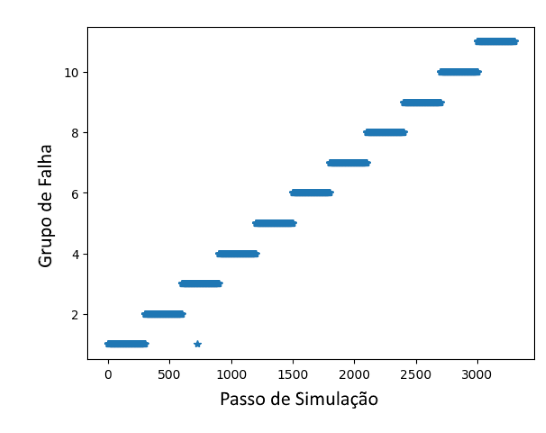
\includegraphics[width=13cm]{./01_Pre_textuais/sallen_figs/GaussianNB_Sallen_Key_mc_+_4bitPRBS_[FALHA]raw.png}
        \caption{\label{fig:GaussianNBClassifieSalenkey}- Circuito: Sallen key - Comportamento Predição GaussianNB}
        \end{center}
        \end{figure}
		
A percentual de acerto total é de 99,87\% para o circuito Sallen Key exemplificado na \ref{fig:GaussianNBClassifieSalenkey} e \ref{tab:sallenGND}. 
\newpage

 \item Classificador K vizinhos mais próximos
 
 \begin{table}[ht]
\centering
\begin{tabular}{ccc}
\textbf{Classe} & \textbf{Acerto (\%)} & \textbf{Acurácia (\%)} \\
Classe 1        & 100                  & 100                    \\
Classe 2        & 100                  & 100                    \\
Classe 3        & 100                  & 100                    \\
Classe 4        & 100                  & 100                    \\
Classe 5        & 100                  & 100                    \\
Classe 6        & 99,9                  & 99,9                    \\
Classe 7        & 100                  & 100                    \\
Classe 8        & 100                  & 100                    \\
Classe 9        & 100                  & 100                    \\
Classe 10       & 100                  & 100                    \\
Classe 11       & 98                  & 98                                 
\end{tabular}
\caption{\label{tab:sallenKvizinhos}- Sallen Key: Falhas K vizinhos}
\end{table}


  \begin{figure}[H]
        \begin{center}
        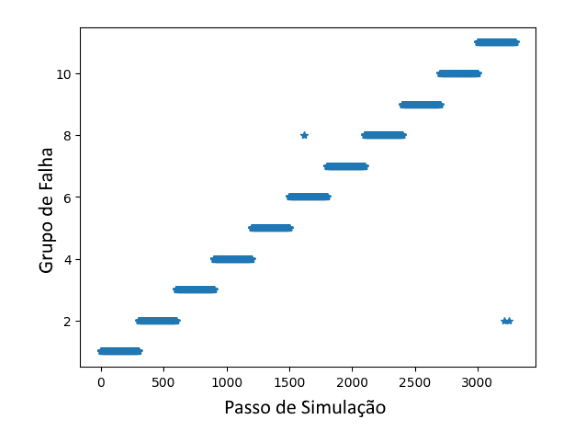
\includegraphics[width=13cm]{./01_Pre_textuais/sallen_figs/KNeighborsClassifier_Sallen_Key_mc_+_4bitPRBS_[FALHA]raw.png}
        \caption{\label{fig:KNeighborsClassifieSalenkey}- Circuito: Sallen key - Comportamento da Predição K Neighbors }
        \end{center}
        \end{figure}

A percentual de acerto total é de 99,8\% para o circuito Sallen Key exemplificado na \ref{fig:KNeighborsClassifieSalenkey} e \ref{tab:sallenKvizinhos}. 
\newpage

 \item Classificador Gradiente de descida estocástica
 
 \begin{table}[ht]
\centering
\begin{tabular}{ccc}
\textbf{Classe} & \textbf{Acerto (\%)} & \textbf{Acurácia (\%)} \\
Classe 1        & 100                  & 100                    \\
Classe 2        & 100                  & 100                    \\
Classe 3        & 100                  & 100                    \\
Classe 4        & 100                  & 100                    \\
Classe 5        & 100                  & 100                    \\
Classe 6        & 100                  & 100                    \\
Classe 7        & 100                  & 100                    \\
Classe 8        & 100                  & 100                    \\
Classe 9        & 100                  & 100                    \\
Classe 10       & 100                  & 100                    \\
Classe 11       & 100                  & 100                                   
\end{tabular}
\caption{\label{tab:sallenGDE}- Sallen Key: Falhas Gradiente de descida estocástica}
\end{table}

 \begin{figure}[H]
        \begin{center}
        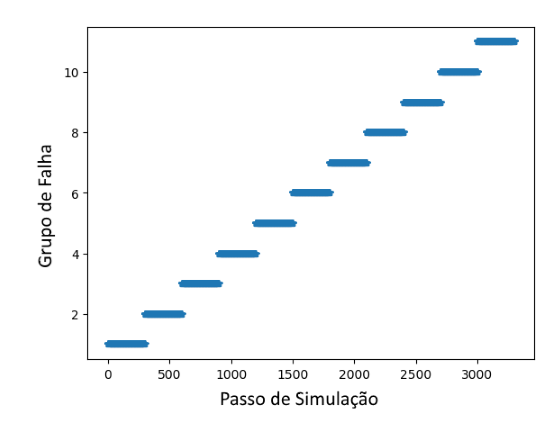
\includegraphics[width=13cm]{./01_Pre_textuais/sallen_figs/SGDClassifier_Sallen_Key_mc_+_4bitPRBS_[FALHA]raw.png}
        \caption{\label{fig:SGDCClassifieSalenkey}- Circuito: Sallen key - Comportamento da Predição SGD}
        \end{center}
        \end{figure}
A percentual de acerto total é de 100\% para o circuito Sallen Key exemplificado na \ref{fig:SGDCClassifieSalenkey} e \ref{tab:sallenGDE}. 

\newpage
 \item Classificador de Regressão logística 
 
 \begin{table}[ht]
\centering
\begin{tabular}{ccc}
\textbf{Classe} & \textbf{Acerto (\%)} & \textbf{Acurácia (\%)} \\
Classe 1        & 100                  & 100                    \\
Classe 2        & 100                  & 100                    \\
Classe 3        & 100                  & 100                    \\
Classe 4        & 100                  & 100                    \\
Classe 5        & 100                  & 100                    \\
Classe 6        & 100                  & 100                    \\
Classe 7        & 100                  & 100                    \\
Classe 8        & 100                  & 100                    \\
Classe 9        & 99                & 99                  \\
Classe 10       & 100                  & 100                    \\
Classe 11       & 100                  & 100                                 
\end{tabular}
\caption{\label{tab:sallenlogistic}- Sallen Key: Falhas Regressão logística}
\end{table}


  \begin{figure}[H]
        \begin{center}
        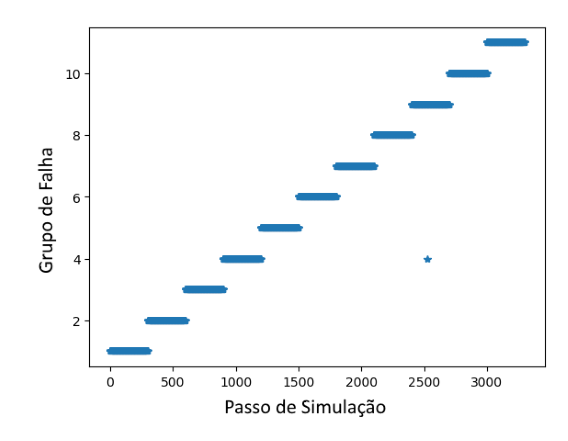
\includegraphics[width=12.5cm]{./01_Pre_textuais/sallen_figs/LogisticRegression_Sallen_Key_mc_+_4bitPRBS_[FALHA]raw.png}
        \caption{\label{fig:LogisticRegressionClassifieSalenkey}- Circuito: Sallen key - Comportamento da Predição regressão Logística }
        \end{center}
        \end{figure}



A percentual de acerto total é de 99,9\% para o circuito Sallen Key exemplificado na \ref{fig:LogisticRegressionClassifieSalenkey} e \ref{tab:sallenlogistic}. 


\end{itemize} 







\section{\textbf{Filtro Passa Alta}}


 Nas imagens a seguir temos o gráfico do estágio inicial. A  \ref{fig:dadobiinicial} exibe os recém adquiridos, mas já manipulado e limpo, ou seja, após o tratamento inicial. 
        
   \begin{figure}[H]
        \begin{center}
        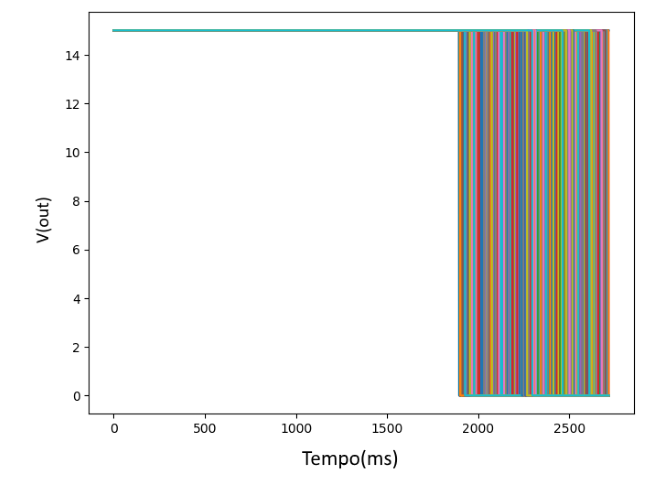
\includegraphics[width=13cm]{./01_Pre_textuais/biquad_figs/dadosPreProc_Biquad_Highpass_Filter_mc_+_4bitPRBS_[FALHA]raw.png}
        \caption{\label{fig:dadobiinicial}- Circuito: Biquad - Dados iniciais}
        \end{center}
        \end{figure}
        
Após a aplicação de PAA e PCA temos um conjunto de dados com apenas 5\% dos dados originais. A \ref{fig:pcabi} exibe os dados limpos e antes de entrar no classificador.

 \begin{figure}[H]
        \begin{center}
        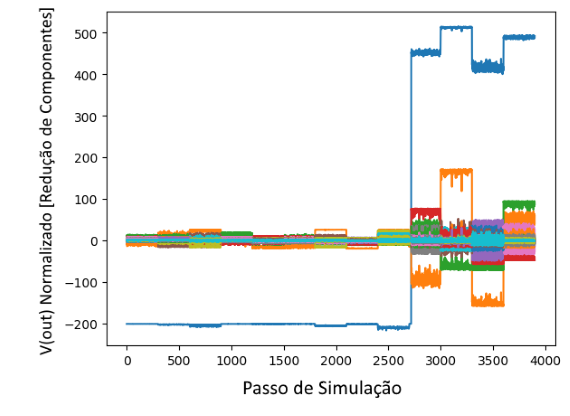
\includegraphics[width=13cm]{./01_Pre_textuais/biquad_figs/PCA_Biquad_Highpass_Filter_mc_+_4bitPRBS_[FALHA]raw.png}
        \caption{\label{fig:pcabi}- Circuito: Biquad - Dados após processamento}
        \end{center}
        \end{figure}
        
O sistema é classificado com oito métodos diferentes descritos anteriormente e com as falhas determinadas na \ref{tab:falhasckt2}. 

A seguir descrevemos a taxa de acerto para cada um dos algoritmos. 


\begin{itemize}
\newpage
 \item Classificador por Árvore de decisão
 
\begin{table}[ht]
\centering
\begin{tabular}{ccc}
\textbf{Classe} & \textbf{Acerto (\%)} & \textbf{Acurácia (\%)} \\
Classe 1        & 100                  & 100                    \\
Classe 2        & 0                  & 0                    \\
Classe 3        & 0                  & 0                    \\
Classe 4        & 0                  & 0                    \\
Classe 5        & 0                  & 0                    \\
Classe 6        & 0                  & 0                    \\
Classe 7        & 0                  & 0                    \\
Classe 8        & 0                  & 0                    \\
Classe 9        & 0                  & 0                    \\
Classe 10       & 0                  & 0                    \\
Classe 11       & 0                  & 0                                       
\end{tabular}
\caption{\label{tab:Biqnarvore}- Biquad: Falhas Árvore de decisão}
\end{table}

 \begin{figure}[H]
        \begin{center}
        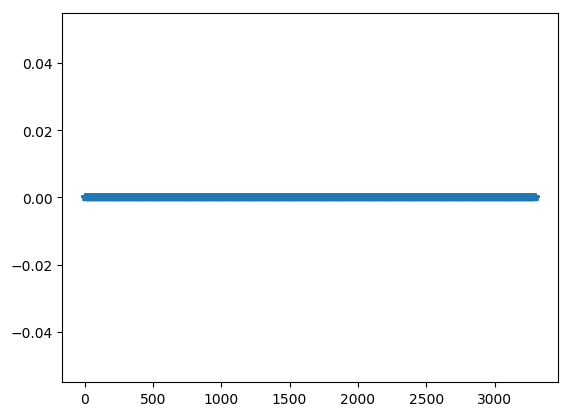
\includegraphics[width=13cm]{./01_Pre_textuais/biquad_figs/DecisionTreeClassifier_Biquad_Highpass_Filter_mc_+_4bitPRBS_[FALHA]raw.png}
        \caption{\label{fig:DecisionTreeClassifieBiq}- Circuito: Biquad - Comportamento da Predição Árvore de decisão}
        \end{center}
        \end{figure}

A percentual de acerto total é de 9\% para o circuito Biquad exemplificado na \ref{fig:DecisionTreeClassifieBiq} e \ref{tab:Biqnarvore}. 
\newpage
 \item Classificador AdaBoost
 
 \begin{table}[ht]
\centering
\begin{tabular}{ccc}
\textbf{Classe} & \textbf{Acerto (\%)} & \textbf{Acurácia (\%)} \\
Classe 1        & 74,2                  & 75                    \\
Classe 2        & 92,42                  & 93                    \\
Classe 3        & 84,69                  & 83,4                    \\
Classe 4        & 62,4                  & 62,4                    \\
Classe 5        & 36,3                  & 36,5                    \\
Classe 6        & 45,4                  & 45,5                    \\
Classe 7        & 93,9                  & 94                    \\
Classe 8        & 99,4                  & 99,5                    \\
Classe 9        & 99,3                 & 99                    \\
Classe 10       & 100                  & 100                    \\
Classe 11       & 100                  & 100                               
\end{tabular}
\caption{\label{tab:BiqnAdaBoost}- Biquad: Falhas AdaBoost}
\end{table}


 \begin{figure}[H]
        \begin{center}
        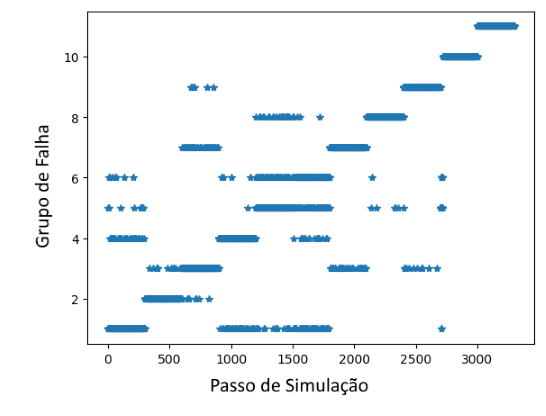
\includegraphics[width=13cm]{./01_Pre_textuais/biquad_figs/AdaBoostClassifier_Biquad_Highpass_Filter_mc_+_4bitPRBS_[FALHA]raw.png}
        \caption{\label{fig:AdaboostClassifieBiq}- Circuito: Biquad - Comportamento da Predição Ada Boost }
        \end{center}
        \end{figure}
       

A percentual de acerto total é de 80,72\% para o circuito Biquad exemplificado na \ref{fig:AdaboostClassifieBiq} e \ref{tab:BiqnAdaBoost}. 

\newpage
 \item Classificador Máquinas de vetores de suporte
 
 \begin{table}[ht]
\centering
\begin{tabular}{ccc}
\textbf{Classe} & \textbf{Acerto (\%)} & \textbf{Acurácia (\%)} \\
Classe 1        & 0                  & 0                    \\
Classe 2        & 0                  & 0                    \\
Classe 3        & 0                  & 0                    \\
Classe 4        & 0                  & 0                    \\
Classe 5        & 0                  & 0                    \\
Classe 6        & 0                  & 0                    \\
Classe 7        & 78,7                  & 79                    \\
Classe 8        & 100                  & 100                    \\
Classe 9        & 0                  & 0                    \\
Classe 10       & 0                  & 0                    \\
Classe 11       & 100                  & 100                               
\end{tabular}
\caption{\label{tab:Biqnsvm}- Biquad: Falhas SVC}
\end{table}

\begin{figure}[H]
        \begin{center}
        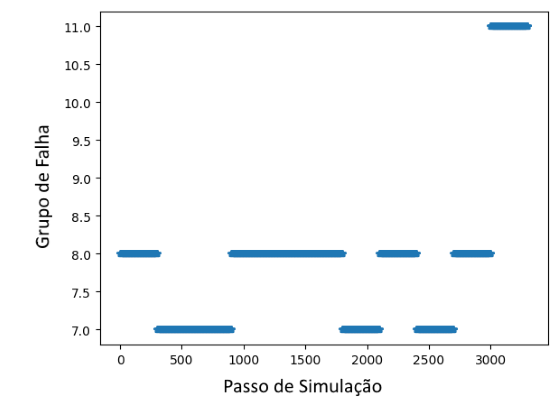
\includegraphics[width=13cm]{./01_Pre_textuais/biquad_figs/SVC_Biquad_Highpass_Filter_mc_+_4bitPRBS_[FALHA]raw.png}
        \caption{\label{fig:SVCClassifieBiq}- Circuito: Biquad - Comportamento da Predição SVC}
        \end{center}
        \end{figure}
       

A percentual de acerto total é de 25,33\% para o circuito Biquad exemplificado na \ref{fig:SVCClassifieBiq} e \ref{tab:Biqnsvm}. 

\newpage

 \item Classificador Floresta aleatória
 
 \begin{table}[ht]
\centering
\begin{tabular}{ccc}
\textbf{Classe} & \textbf{Acerto (\%)} & \textbf{Acurácia (\%)} \\
Classe 1        & 96,7                 & 95,5                   \\
Classe 2        & 77,4                  & 77,4                    \\
Classe 3        & 40,7                  & 40,7                    \\
Classe 4        & 63,6                  & 63,7                    \\
Classe 5        & 34,72                  & 35                    \\
Classe 6        & 44,42                  & 44,5                   \\
Classe 7        & 99,3                  & 99,4                      \\
Classe 8        & 96,9                  & 96,5                 \\
Classe 9        & 100                  & 100                    \\
Classe 10       & 100                  & 100                    \\
Classe 11       & 100                  & 100                                  
\end{tabular}
\caption{\label{tab:Biqnrandom}- Biquad: Falhas Floresta aleatória}
\end{table}


  \begin{figure}[H]
        \begin{center}
        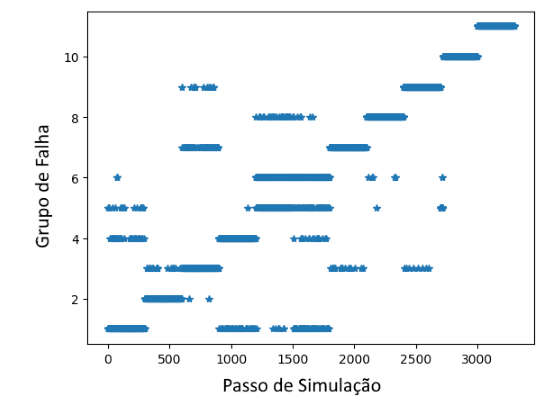
\includegraphics[width=13cm]{./01_Pre_textuais/biquad_figs/RandomForestClassifier_Biquad_Highpass_Filter_mc_+_4bitPRBS_[FALHA]raw.png}
        \caption{\label{fig:randomforestClassifieBiq}- Circuito: Biquad - Comportamento da Predição Random Forest }
        \end{center}
        \end{figure}

A percentual de acerto total é de 77,55\% para o circuito Biquad exemplificado na \ref{fig:randomforestClassifieBiq} e \ref{tab:Biqnrandom}. 

\newpage
 \item Classificador Gaussiano de Naive Bayes
 
 \begin{table}[ht]
\centering
\begin{tabular}{ccc}
\textbf{Classe} & \textbf{Acerto (\%)} & \textbf{Acurácia (\%)} \\
Classe 1        & 76,8                  & 83,9                   \\
Classe 2        & 89,5                  & 97,3                    \\
Classe 3        & 62,8                  & 86,4                    \\
Classe 4        & 83,8                  & 76,5                    \\
Classe 5        & 53,5                  & 83,7                    \\
Classe 6        & 44,42                & 37,8                    \\
Classe 7        & 92,5                  & 74,9                    \\
Classe 8        & 98,9                  & 94,7                    \\
Classe 9        & 98,36            & 99,4                   \\
Classe 10       & 100                  & 99                    \\
Classe 11       & 100                  & 100                                 
\end{tabular}
\caption{\label{tab:BiqnGND}- Biquad: Falhas Gaussiano de Naive Bayes}
\end{table}


  \begin{figure}[H]
        \begin{center}
        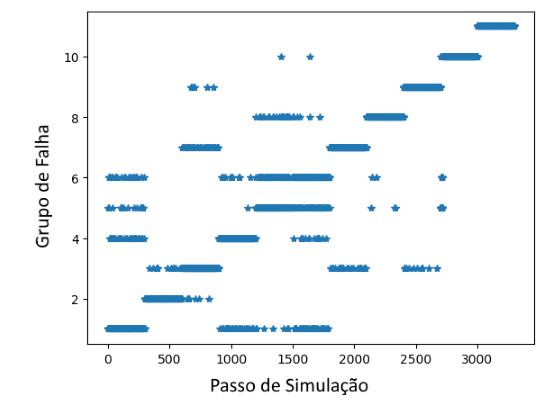
\includegraphics[width=13cm]{./01_Pre_textuais/biquad_figs/GaussianNB_Biquad_Highpass_Filter_mc_+_4bitPRBS_[FALHA]raw.png}
        \caption{\label{fig:GaussianNBClassifieBiq}- Circuito: Biquad - Comportamento Predição GaussianNB}
        \end{center}
        \end{figure}
		
A percentual de acerto total é de 81.87\% para o circuito Biquad exemplificado na \ref{fig:GaussianNBClassifieBiq} e \ref{tab:BiqnGND}. 
\newpage

 \item Classificador K vizinhos mais próximos
 
 \begin{table}[ht]
\centering
\begin{tabular}{ccc}
\textbf{Classe} & \textbf{Acerto (\%)} & \textbf{Acurácia (\%)} \\
Classe 1        & 98                   & 61,8                    \\
Classe 2        & 97,4                  & 91,2                    \\
Classe 3        & 48,6                  & 79,3                    \\
Classe 4        & 56,78                  & 92,4                    \\
Classe 5        & 45,5                  & 98,3                    \\
Classe 6        & 38,2                  & 44,4                    \\
Classe 7        & 97,1                  & 74,2                    \\
Classe 8        & 99,3                  & 96,4                    \\
Classe 9        & 99,6                  & 94,3                    \\
Classe 10       & 100                  & 99,9                    \\
Classe 11       & 99,9                  & 100                                 
\end{tabular}
\caption{\label{tab:BiqnKvizinhos}- Biquad: Falhas K vizinhos}
\end{table}


  \begin{figure}[H]
        \begin{center}
        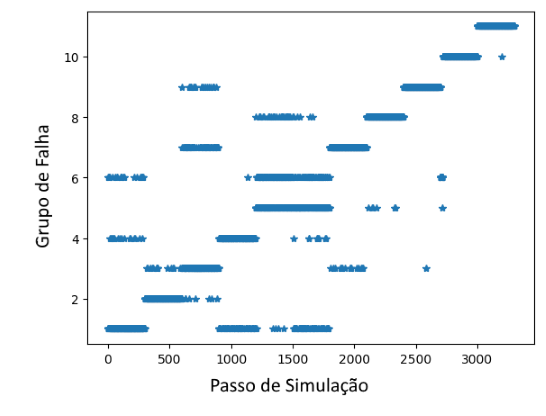
\includegraphics[width=13cm]{./01_Pre_textuais/biquad_figs/KNeighborsClassifier_Biquad_Highpass_Filter_mc_+_4bitPRBS_[FALHA]raw.png}
        \caption{\label{fig:KNeighborsClassifieBiq}- Circuito: Biquad - Comportamento da Predição K Neighbors }
        \end{center}
        \end{figure}

A percentual de acerto total é de 80\% para o circuito Biquad exemplificado na \ref{fig:KNeighborsClassifieBiq} e \ref{tab:BiqnKvizinhos}. 
\newpage

 \item Classificador Gradiente de descida estocástica
 
 \begin{table}[ht]
\centering
\begin{tabular}{ccc}
\textbf{Classe} & \textbf{Acerto (\%)} & \textbf{Acurácia (\%)} \\
Classe 1        & 87,2                  & 91                   \\
Classe 2        & 97,4                  & 99,8                   \\
Classe 3        & 74,8                  & 89,6                    \\
Classe 4        & 64,3                  & 78,8                    \\
Classe 5        & 73,2                  & 94,3                    \\
Classe 6        & 51,4                  & 48,8                    \\
Classe 7        & 98,7                  & 67,4                    \\
Classe 8        & 99,3                  & 84,2                    \\
Classe 9        & 99,5                  & 99,7                    \\
Classe 10       & 100                  & 100                    \\
Classe 11       & 100                  & 100                                   
\end{tabular}
\caption{\label{tab:BiqnGDE}- Biquad: Falhas Gradiente de descida estocástica}
\end{table}

 \begin{figure}[H]
        \begin{center}
        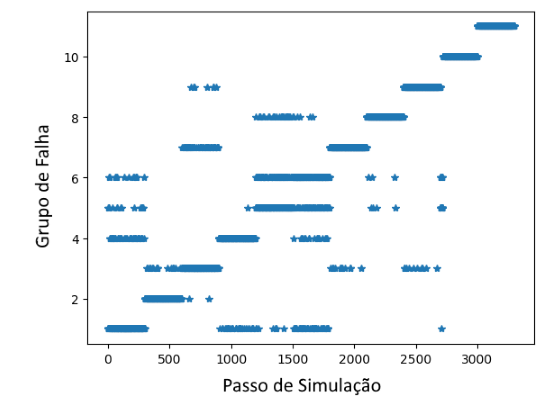
\includegraphics[width=13cm]{./01_Pre_textuais/biquad_figs/SGDClassifier_Biquad_Highpass_Filter_mc_+_4bitPRBS_[FALHA]raw.png}
        \caption{\label{fig:SGDCClassifieBiq}- Circuito: Biquad - Comportamento da Predição SGD}
        \end{center}
        \end{figure}
A percentual de acerto total é de 85,98\% para o circuito Biquad exemplificado na \ref{fig:SGDCClassifieBiq} e \ref{tab:BiqnGDE}. 

\newpage
 \item Classificador de Regressão logística 
 
 \begin{table}[ht]
\centering
\begin{tabular}{ccc}
\textbf{Classe} & \textbf{Acerto (\%)} & \textbf{Acurácia (\%)} \\
Classe 1        & 62,2                  & 86,1                    \\
Classe 2        & 98,3                  & 99,3                    \\
Classe 3        & 36,8                  & 86,2                    \\
Classe 4        & 77,1                  & 51,2                    \\
Classe 5        & 56,8                  & 32,7                    \\
Classe 6        & 0                  & 0                    \\
Classe 7        & 99,8                  & 61,3                   \\
Classe 8        & 99,1                  & 99,8                    \\
Classe 9        & 97                  & 99,6                    \\
Classe 10       & 100                  & 100                    \\
Classe 11       & 100                  & 98,2                                 
\end{tabular}
\caption{\label{tab:Biqnlogistic}- Biquad: Falhas Regressão logística}
\end{table}


  \begin{figure}[H]
        \begin{center}
        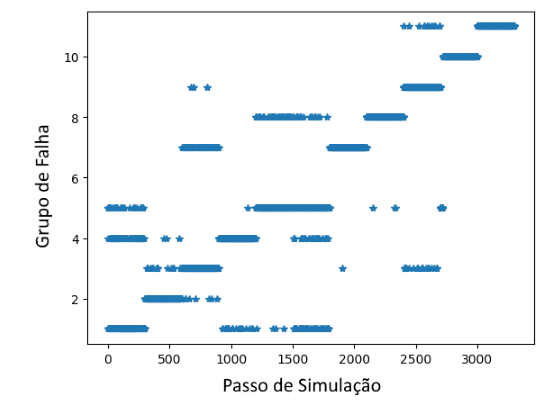
\includegraphics[width=12.5cm]{./01_Pre_textuais/biquad_figs/LogisticRegression_Biquad_Highpass_Filter_mc_+_4bitPRBS_[FALHA]raw.png}
        \caption{\label{fig:LogisticRegressionClassifieBiq}- Circuito: Biquad - Comportamento da Predição regressão Logística }
        \end{center}
        \end{figure}

A percentual de acerto total é de 78,53\% para o circuito Biquad exemplificado na \ref{fig:LogisticRegressionClassifieBiq} e \ref{tab:Biqnlogistic}. 


\end{itemize} 

\section{\textbf{Filtro universal}}


 Nas imagens a seguir temos o gráfico do estágio inicial. A  \ref{fig:dadoCSTVinicial} exibe os recém adquiridos, mas já manipulado e limpo, ou seja, após o tratamento inicial. 
  
  \begin{figure}[H]
        \begin{center}
        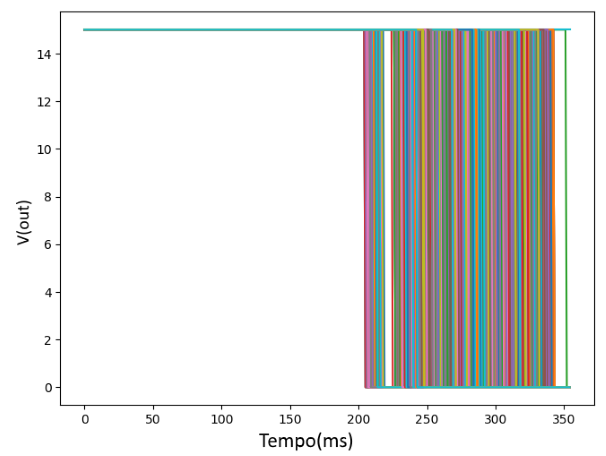
\includegraphics[width=13cm]{./01_Pre_textuais/ctsv_figs/dadosPreProc_CTSV_mc_+_4bitPRBS_[FALHA]raw.png}
        \caption{\label{fig:dadoCSTVinicial}- Circuito: CTSV - Dados iniciais}
        \end{center}
        \end{figure}
        

Após a aplicação de PAA e PCA temos um conjunto de dados com apenas 5\% dos dados originais. A \ref{fig:pcacstv} exibe os dados limpos e antes de entrar no classificador.

\begin{figure}[H]
        \begin{center}
        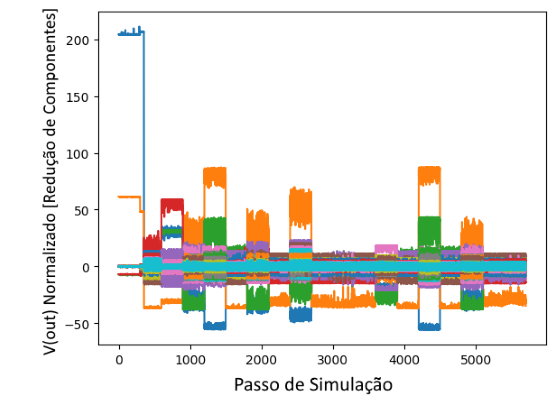
\includegraphics[width=13cm]{./01_Pre_textuais/ctsv_figs/PCA_CTSV_mc_+_4bitPRBS_[FALHA]raw.png}
        \caption{\label{fig:pcacstv}- Circuito: CTSV  - Dados após processamento}
        \end{center}
        \end{figure}

O sistema é classificado com oito métodos diferentes descritos anteriormente e com as falhas determinadas na \ref{tab:falhasckt3}. 

A seguir descrevemos a taxa de acerto para cada um dos algoritmos. 
\newpage

\begin{itemize}

 \item Classificador por Árvore de decisão
 
\begin{table}[ht]
\centering
\begin{tabular}{ccc}
\textbf{Classe} & \textbf{Acerto (\%)} & \textbf{Acurácia (\%)} \\
Classe 1        & 100                  & 5,2                    \\
Classe 2        & 0                 & 0                   \\
Classe 3       & 0                 & 0                     \\
Classe 4       & 0                 & 0                     \\
Classe 5        & 0                 & 0                     \\
Classe 6        & 0                 & 0                      \\
Classe 7        & 0                 & 0                      \\
Classe 8        & 0                 & 0                     \\
Classe 9        & 0                 & 0                     \\
Classe 10       & 0                 & 0                     \\
Classe 11      & 0                 & 0      
     \\
Classe 12       & 0                 & 0   
     \\
Classe 13      & 0                 & 0    
     \\
Classe 14       & 0                 & 0   
     \\
Classe 15       & 0                 & 0    
     \\
Classe 16       & 0                 & 0   
     \\
Classe 17       & 0                 & 0   
     \\
Classe 18     & 0                 & 0    
     \\
Classe 19       & 0                 & 0   
\end{tabular}
\caption{\label{tab:ctsvnarvore}- CTSV: Falhas Árvore de decisão}
\end{table}

 \begin{figure}[H]
        \begin{center}
        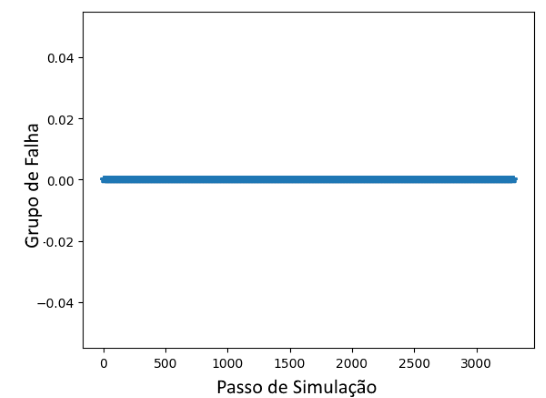
\includegraphics[width=11cm]{./01_Pre_textuais/ctsv_figs/DecisionTreeClassifier_CTSV_mc_+_4bitPRBS_[FALHA]raw.png}
        \caption{\label{fig:DecisionTreeClassifiectsv}- Circuito: CTSV - Comportamento da Predição Árvore de decisão}
        \end{center}
        \end{figure}

A percentual de acerto total é de 5,2\% para o circuito CTSV exemplificado na \ref{fig:DecisionTreeClassifiectsv} e \ref{tab:ctsvnarvore}. 
\newpage
 \item Classificador AdaBoost
 
 \begin{table}[ht]
\centering
\begin{tabular}{ccc}
\textbf{Classe} & \textbf{Acerto (\%)} & \textbf{Acurácia (\%)} \\
Classe 1        & 100                  & 100                    \\
Classe 2        & 95,6                  & 91,2                    \\
Classe 3        & 89,2                  & 100                    \\
Classe 4        & 58,1                  & 62,5                    \\
Classe 5        & 89,2                 & 98,2                    \\
Classe 6        & 63,4                  & 82,7                    \\
Classe 7        & 73,8                  & 48,9                    \\
Classe 8        & 76                  & 39                    \\
Classe 9        & 87                  & 93,9                    \\
Classe 10       & 0                  & 0                    \\
Classe 11       & 75,8            & 100   
     \\
Classe 12       & 0                 & 0   
     \\
Classe 13      & 21,8                 & 12    
     \\
Classe 14       &  75,9                & 56,8   
     \\
Classe 15       & 95                 & 94
     \\
Classe 16       & 52,9                &    76,8
     \\
Classe 17       & 65,9                & 21,7
     \\
Classe 18     &  67,4              &    65,8 
     \\
Classe 19       & 72,8                 & 73,1   
\end{tabular}
\caption{\label{tab:ctsvnAdaBoost}- CTSV: Falhas AdaBoost}
\end{table}


 \begin{figure}[H]
        \begin{center}
        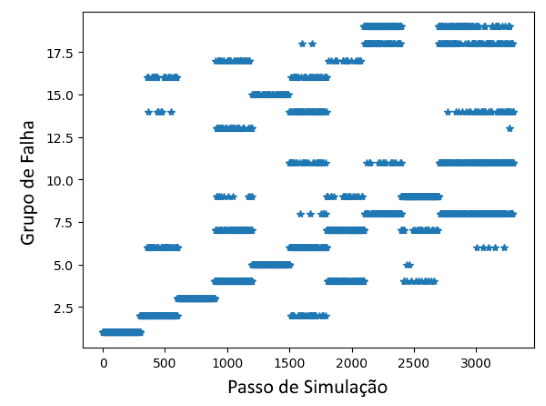
\includegraphics[width=11cm]{./01_Pre_textuais/ctsv_figs/AdaBoostClassifier_CTSV_mc_+_4bitPRBS_[FALHA]raw.png}
        \caption{\label{fig:AdaboostClassifiectsv}- Circuito: CTSV - Comportamento da Predição AdaBoost }
        \end{center}
        \end{figure}
       

A percentual de acerto total é de 66,3\% para o circuito CTSV exemplificado na \ref{fig:AdaboostClassifiectsv} e \ref{tab:ctsvnAdaBoost}. 

\newpage
 \item Classificador Máquinas de vetores de suporte
 
 \begin{table}[ht]
\centering
\begin{tabular}{ccc}
\textbf{Classe} & \textbf{Acerto (\%)} & \textbf{Acurácia (\%)} \\
Classe 1        & 100                  & 100                    \\
Classe 2        & 0                  & 0                    \\
Classe 3        & 100                  & 100                    \\
Classe 4        & 0                  & 0                    \\
Classe 5        & 0                  & 0                    \\
Classe 6        & 0                  & 0                    \\
Classe 7        & 0                  & 0                    \\
Classe 8        & 0                  & 0                    \\
Classe 9        & 100                  & 98                    \\
Classe 10       & 0                  & 0                    \\
Classe 11       & 87                  & 22,4 
\\
Classe 12       & 0                 & 0   
     \\
Classe 13      & 0                 & 0    
     \\
Classe 14       & 0                 & 0   
     \\
Classe 15       & 0                 & 0    
     \\
Classe 16       & 0                 & 0   
     \\
Classe 17       & 0                 & 0   
     \\
Classe 18     & 0                 & 0    
     \\
Classe 19       & 0                 & 0   
\end{tabular}
\caption{\label{tab:ctsvnsvm}- CTSV: Falhas SVC}
\end{table}

\begin{figure}[H]
        \begin{center}
        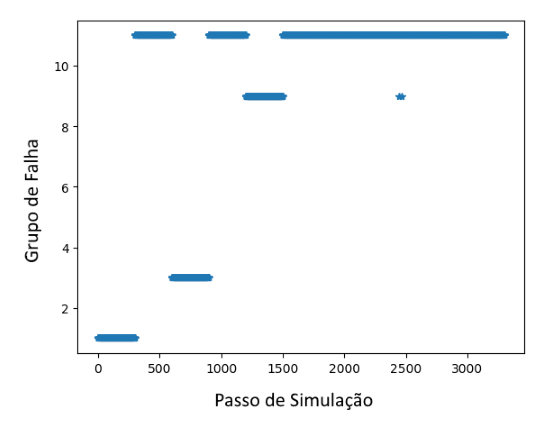
\includegraphics[width=11cm]{./01_Pre_textuais/ctsv_figs/SVC_CTSV_mc_+_4bitPRBS_[FALHA]raw.png}
        \caption{\label{fig:SVCClassifiectsv}- Circuito: CTSV - Comportamento da Predição SVC}
        \end{center}
        \end{figure}
       

A percentual de acerto total é de 20,36\% para o circuito CTSV exemplificado na \ref{fig:SVCClassifiectsv} e \ref{tab:ctsvnsvm}. 

\newpage

 \item Classificador Floresta aleatória
 
 \begin{table}[ht]
\centering
\begin{tabular}{ccc}
\textbf{Classe} & \textbf{Acerto (\%)} & \textbf{Acurácia (\%)} \\
Classe 1        & 100                  & 100                    \\
Classe 2        & 95,6                  & 91,2                    \\
Classe 3        & 86,2                  & 100                    \\
Classe 4        & 58,1                  & 62,5                    \\
Classe 5        & 89,2                 & 98,2                    \\
Classe 6        & 63,4                  & 82,7                    \\
Classe 7        & 73,8                  & 48,9                    \\
Classe 8        & 79.8                  & 39                    \\
Classe 9        & 87                  & 93,9                    \\
Classe 10       & 0                  & 0                    \\
Classe 11       & 79,8            & 100   
     \\
Classe 12       & 0                 & 0   
     \\
Classe 13      & 21,8                 & 12    
     \\
Classe 14       &  75,9                & 56,8   
     \\
Classe 15       & 95                 & 94
     \\
Classe 16       & 52,9                &    76,8
     \\
Classe 17       & 60,3                & 21,7
     \\
Classe 18     &  67,4              &    65,8 
     \\
Classe 19       & 79,8                 & 73,1    

\end{tabular}
\caption{\label{tab:ctsvnrandom}- CTSV: Falhas Floresta aleatória}
\end{table}


  \begin{figure}[H]
        \begin{center}
        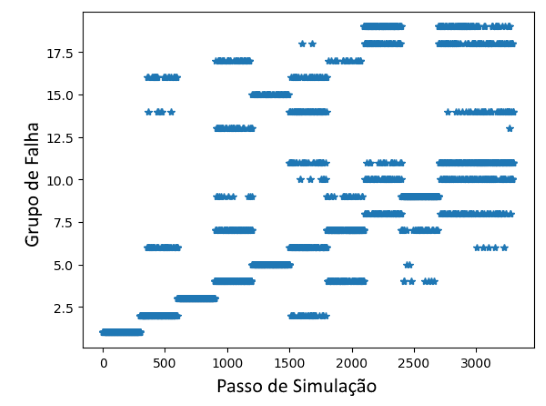
\includegraphics[width=11cm]{./01_Pre_textuais/ctsv_figs/RandomForestClassifier_CTSV_mc_+_4bitPRBS_[FALHA]raw.png}
        \caption{\label{fig:randomforestClassifiectsv}- Circuito: CTSV - Comportamento da Predição Random Forest }
        \end{center}
        \end{figure}

A percentual de acerto total é de 66,63\% para o circuito CTSV exemplificado na \ref{fig:randomforestClassifiectsv} e \ref{tab:ctsvnrandom}. 

\newpage
 \item Classificador Gaussiano de Naive Bayes
 
 \begin{table}[ht]
\centering
\begin{tabular}{ccc}
\textbf{Classe} & \textbf{Acerto (\%)} & \textbf{Acurácia (\%)} \\
Classe 1        & 100                  & 100                    \\
Classe 2        & 95,6                  & 95,2                    \\
Classe 3        & 86,2                  & 100                    \\
Classe 4        & 58,1                  & 67,5                    \\
Classe 5        & 83,2                 & 98,2                    \\
Classe 6        & 63,4                  & 82,7                    \\
Classe 7        & 73,2                  & 48,9                    \\
Classe 8        & 79.8                  & 37,9                    \\
Classe 9        & 82.8                  & 94,9                    \\
Classe 10       & 0                  & 0                    \\
Classe 11       & 81,8            & 89,9   
     \\
Classe 12       & 0                 & 0   
     \\
Classe 13      & 24,8                 & 13,4    
     \\
Classe 14       &  75,9                & 56,8   
     \\
Classe 15       & 93,7                 & 94
     \\
Classe 16       & 59,9                &    76,8
     \\
Classe 17       & 57,3                & 21,7
     \\
Classe 18     &  68,4              &    62,8 
     \\
Classe 19       & 77,8                 & 73,1                                 
\end{tabular}
\caption{\label{tab:ctsvnGND}- CTSV: Falhas Gaussiano de Naive Bayes}
\end{table}


  \begin{figure}[H]
        \begin{center}
        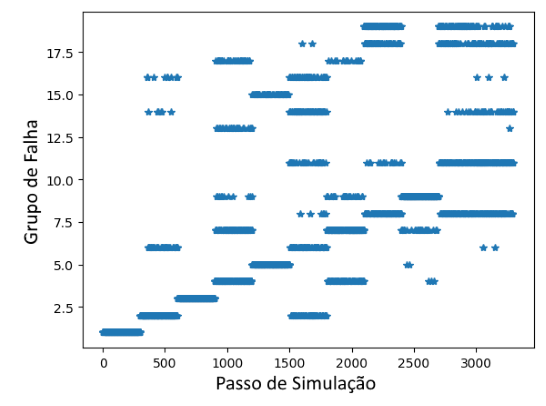
\includegraphics[width=11cm]{./01_Pre_textuais/ctsv_figs/GaussianNB_CTSV_mc_+_4bitPRBS_[FALHA]raw.png}
        \caption{\label{fig:GaussianNBClassifiectsv}- Circuito: CTSV - Comportamento Predição GaussianNB}
        \end{center}
        \end{figure}
		
A percentual de acerto total é de 66,39\% para o circuito CTSV exemplificado na \ref{fig:GaussianNBClassifiectsv} e \ref{tab:ctsvnGND}. 
\newpage

 \item Classificador K vizinhos mais próximos
 
 \begin{table}[ht]
\centering
\begin{tabular}{ccc}
\textbf{Classe} & \textbf{Acerto (\%)} & \textbf{Acurácia (\%)} \\
Classe 1        & 99,8                  & 100                    \\
Classe 2        & 92,6                  & 99,2                    \\
Classe 3        & 86,2                  & 100                    \\
Classe 4        & 0                  & 0                    \\
Classe 5        & 89,8                 & 98,2                    \\
Classe 6        & 68,4                  & 82,7                    \\
Classe 7        & 73,8                  & 48,9                    \\
Classe 8        & 79.8                  & 39                    \\
Classe 9        & 87                  & 93,9                    \\
Classe 10       & 17                  & 76                    \\
Classe 11       & 79,8            & 100   
     \\
Classe 12       & 0                 & 0   
     \\
Classe 13      & 21,8                 & 12    
     \\
Classe 14       &  78,9                & 56,8   
     \\
Classe 15       & 56                 & 94
     \\
Classe 16       & 76,9                &    76,8
     \\
Classe 17       & 19,3                & 21,7
     \\
Classe 18     &  42,4              &    65,8 
     \\
Classe 19       & 39,8                 & 73,1                                
\end{tabular}
\caption{\label{tab:ctsvnKvizinhos}- CTSV: Falhas K vizinhos}
\end{table}


  \begin{figure}[H]
        \begin{center}
        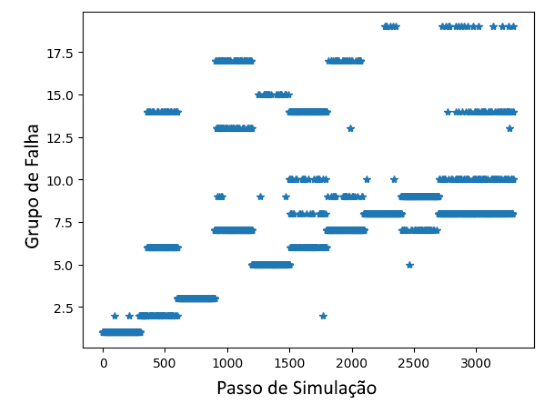
\includegraphics[width=11cm]{./01_Pre_textuais/ctsv_figs/KNeighborsClassifier_CTSV_mc_+_4bitPRBS_[FALHA]raw.png}
        \caption{\label{fig:KNeighborsClassifiectsv}- Circuito: CTSV - Comportamento da Predição K Neighbors }
        \end{center}
        \end{figure}

A percentual de acerto total é de 58,38\% para o circuito CTSV exemplificado na \ref{fig:KNeighborsClassifiectsv} e \ref{tab:ctsvnKvizinhos}. 
\newpage

 \item Classificador Gradiente de descida estocástica
 
 \begin{table}[ht]
\centering
\begin{tabular}{ccc}
\textbf{Classe} & \textbf{Acerto (\%)} & \textbf{Acurácia (\%)} \\
Classe 1        & 100                  & 100                    \\
Classe 2        & 68,6                  & 56,2                    \\
Classe 3        & 86,2                  & 100                    \\
Classe 4        & 78,1                  & 62,5                    \\
Classe 5        & 89,2                 & 98,2                    \\
Classe 6        & 63,4                  & 82,7                    \\
Classe 7        & 73,8                  & 87,9                    \\
Classe 8        & 79.8                  & 89                    \\
Classe 9        & 67.9                  & 93,9                    \\
Classe 10       & 0                  & 0                    \\
Classe 11       & 88,8            & 76   
     \\
Classe 12       & 67,9                 & 85,4   
     \\
Classe 13      & 21,8                 & 12    
     \\
Classe 14       &  75,9                & 56,8   
     \\
Classe 15       & 95                 & 94
     \\
Classe 16       & 52,9                &    76,8
     \\
Classe 17       & 60,3                & 21,7
     \\
Classe 18     &  57,4              &    65,8 
     \\
Classe 19       & 59,8                 & 73,1                                   
\end{tabular}
\caption{\label{tab:ctsvnGDE}- CTSV: Falhas Gradiente de descida estocástica}
\end{table}

 \begin{figure}[H]
        \begin{center}
        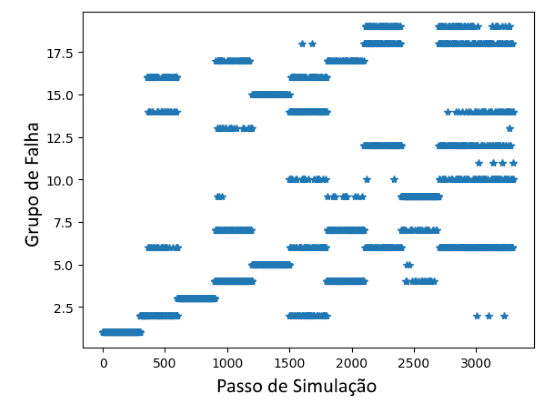
\includegraphics[width=11cm]{./01_Pre_textuais/ctsv_figs/SGDClassifier_CTSV_mc_+_4bitPRBS_[FALHA]raw.png}
        \caption{\label{fig:SGDCClassifiectsv}- Circuito: CTSV - Comportamento da Predição SGD}
        \end{center}
        \end{figure}
A percentual de acerto total é de 84,98\% para o circuito CTSV exemplificado na \ref{fig:SGDCClassifiectsv} e \ref{tab:ctsvnGDE}. 

\newpage
 \item Classificador de Regressão logística 
 
 \begin{table}[ht]
\centering
\begin{tabular}{ccc}
\textbf{Classe} & \textbf{Acerto (\%)} & \textbf{Acurácia (\%)} \\
Classe 1        & 97,5                  & 93,7                    \\
Classe 2        & 85,6                  & 91,2                    \\
Classe 3        & 96,2                  & 100                    \\
Classe 4        & 58,1                  & 62,5                    \\
Classe 5        & 94,2                 & 99,2                    \\
Classe 6        & 76,4                  & 59,7                    \\
Classe 7        & 0                  & 0                    \\
Classe 8        & 0                  & 0                    \\
Classe 9        & 87                  & 93,9                    \\
Classe 10       & 0                  & 0                    \\
Classe 11       & 64,5            & 32,5   
     \\
Classe 12       & 67                 & 75   
     \\
Classe 13      & 21,8                 & 65    
     \\
Classe 14       &  77,9                & 56,8   
     \\
Classe 15       & 95                 & 94
     \\
Classe 16       & 0                &    0
     \\
Classe 17       & 86,3                & 67,7
     \\
Classe 18     &  0              &    0 
     \\
Classe 19       & 0                 & 0                                 
\end{tabular}
\caption{\label{tab:ctsvnlogistic}- CTSV: Falhas Regressão logística}
\end{table}


  \begin{figure}[H]
        \begin{center}
        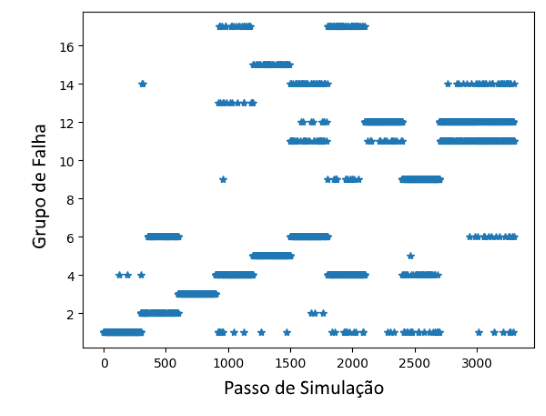
\includegraphics[width=11cm]{./01_Pre_textuais/ctsv_figs/LogisticRegression_CTSV_mc_+_4bitPRBS_[FALHA]raw.png}
        \caption{\label{fig:LogisticRegressionClassifiectsv}- Circuito: CTSV - Comportamento da regressão Logística }
        \end{center}
        \end{figure}

A percentual de acerto total é de 53,02\% para o circuito CTSV exemplificado na \ref{fig:LogisticRegressionClassifiectsv} e \ref{tab:ctsvnlogistic}. 


\end{itemize} 


\section{\textbf{Retificador não linear}}


 Nas imagens a seguir temos o gráfico do estágio inicial. A  \ref{fig:dadoPAAretificador} exibe os recém adquiridos, mas já manipulado e limpo, ou seja, após o tratamento inicial. 
 
\begin{figure}[H]
        \begin{center}
        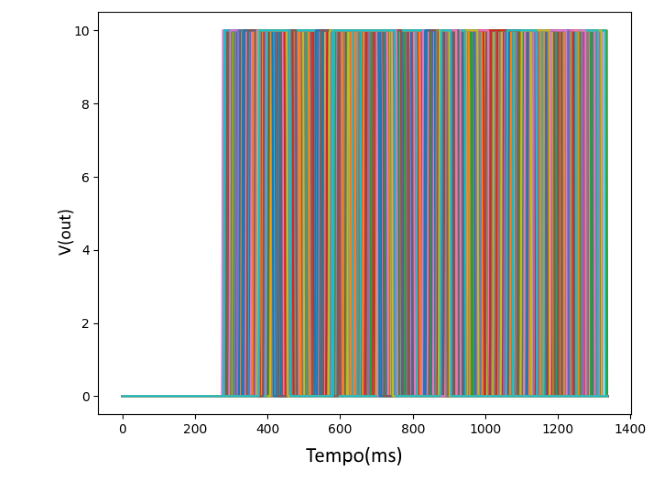
\includegraphics[width=13cm]{./01_Pre_textuais/nonlin_figs/dadosPreProc_Nonlinear_Rectfier_+_4bit_PRBS_[FALHA]_-_300_-_02sraw.png}
        \caption{\label{fig:dadoPAAretificador}- Circuito: Retificador  - Dados iniciais}
        \end{center}
        \end{figure}
        
Após a aplicação de PAA e PCA temos um conjunto de dados com apenas 5\% dos dados originais. A \ref{fig:pcaretificador} exibe os dados limpos e antes de entrar no classificador.

\begin{figure}[H]
        \begin{center}
        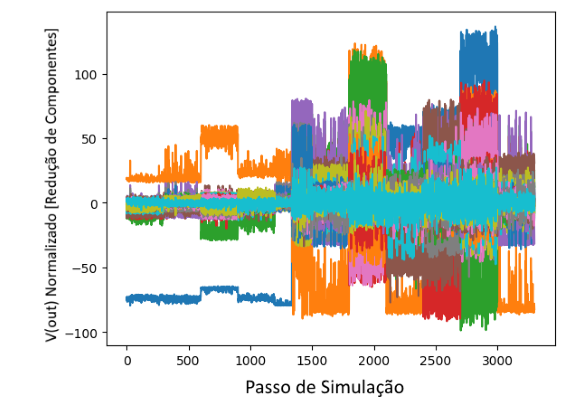
\includegraphics[width=13cm]{./01_Pre_textuais/nonlin_figs/PCA_Nonlinear_Rectfier_+_4bit_PRBS_[FALHA]_-_300_-_02sraw.png}
        \caption{\label{fig:pcaretificador}- Circuito: Retificador - Dados após processamento}
        \end{center}
        \end{figure}

O sistema é classificado com oito métodos diferentes descritos anteriormente e com as falhas determinadas na \ref{tab:falhasckt4}. 

A seguir descrevemos a taxa de acerto para cada um dos algoritmos. 


\begin{itemize}
\newpage
 \item Classificador por Árvore de decisão
 
\begin{table}[ht]
\centering
\begin{tabular}{ccc}
\textbf{Classe} & \textbf{Acerto (\%)} & \textbf{Acurácia (\%)} \\
Classe 1        & 100                  & 9                    \\
Classe 2         & 0                  & 0                    \\
Classe 3        & 0                  & 0                     \\
Classe 4       & 0                  & 0                     \\
Classe 5        & 0                  & 0                    \\
Classe 6        & 0                  & 0                     \\
Classe 7         & 0                  & 0                     \\
Classe 8         & 0                  & 0                      \\
Classe 9         & 0                  & 0                     \\
Classe 10        & 0                  & 0                    \\
Classe 11       & 0                  & 0                                      
\end{tabular}
\caption{\label{tab:Retnarvore}- Retificador: Falhas Árvore de decisão}
\end{table}

 \begin{figure}[H]
        \begin{center}
        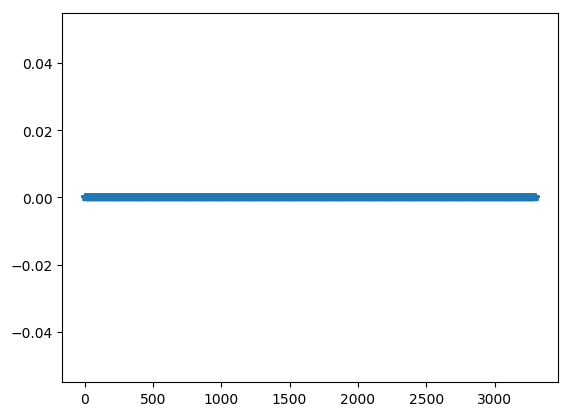
\includegraphics[width=13cm]{./01_Pre_textuais/nonlin_figs/DecisionTreeClassifier_Nonlinear_Rectfier_+_4bit_PRBS_[FALHA]_-_300_-_02sraw.png}
        \caption{\label{fig:DecisionTreeClassifieRet}- Circuito: Retificador - Comportamento da Predição Árvore de decisão}
        \end{center}
        \end{figure}

A percentual de acerto total é de 9\% para o circuito Retificador exemplificado na \ref{fig:DecisionTreeClassifieRet} e \ref{tab:Retnarvore}. 
\newpage
 \item Classificador AdaBoost
 
 \begin{table}[ht]
\centering
\begin{tabular}{ccc}
\textbf{Classe} & \textbf{Acerto (\%)} & \textbf{Acurácia (\%)} \\
Classe 1        & 99,9                  & 99,75                    \\
Classe 2        & 99,84                  & 99,6                    \\
Classe 3        & 100                  & 100                    \\
Classe 4        & 99,87                  & 99,9                    \\
Classe 5        & 99,9                  & 99,8                    \\
Classe 6        & 97,6                  & 97,5                    \\
Classe 7        & 100                  & 100                    \\
Classe 8        & 99,89                  & 99,9                    \\
Classe 9        & 99,9                  & 99,9                    \\
Classe 10       & 99,8                  & 100                    \\
Classe 11       & 98,6                  & 97,6                               
\end{tabular}
\caption{\label{tab:RetnAdaBoost}- Retificador: Falhas AdaBoost}
\end{table}


 \begin{figure}[H]
        \begin{center}
        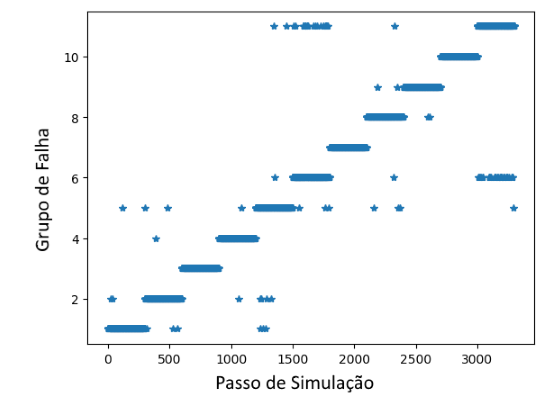
\includegraphics[width=13cm]{./01_Pre_textuais/nonlin_figs/AdaBoostClassifier_Nonlinear_Rectfier_+_4bit_PRBS_[FALHA]_-_300_-_02sraw.png}
        \caption{\label{fig:AdaboostClassifieRet}- Circuito: Retificador - Comportamento da Predição Ada Boost }
        \end{center}
        \end{figure}
       

A percentual de acerto total é de 99,57\% para o circuito Retificador exemplificado na \ref{fig:AdaboostClassifieRet} e \ref{tab:RetnAdaBoost}. 

\newpage
 \item Classificador Máquinas de vetores de suporte
 
 \begin{table}[ht]
\centering
\begin{tabular}{ccc}
\textbf{Classe} & \textbf{Acerto (\%)} & \textbf{Acurácia (\%)} \\
Classe 1        & 100                  & 25,25                    \\
Classe 2        & 0                  & 0                    \\
Classe 3        & 100                  & 100                    \\
Classe 4        & 0                  & 0                    \\
Classe 5        & 0                  & 0                    \\
Classe 6        & 0                  & 0                    \\
Classe 7        & 0                  & 0                    \\
Classe 8        & 0                  & 0                    \\
Classe 9        & 100                  & 36,8                   \\
Classe 10       & 0                  & 0                    \\
Classe 11       & 0                  &  0                              
\end{tabular}
\caption{\label{tab:Retnsvm}- Retificador: Falhas SVC}
\end{table}

\begin{figure}[H]
        \begin{center}
        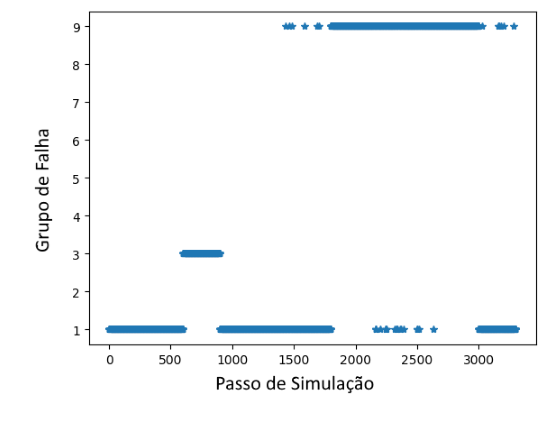
\includegraphics[width=13cm]{./01_Pre_textuais/nonlin_figs/SVC_Nonlinear_Rectfier_+_4bit_PRBS_[FALHA]_-_300_-_02sraw.png}
        \caption{\label{fig:SVCClassifieRet}- Circuito: Retificador - Comportamento da Predição SVC}
        \end{center}
        \end{figure}
       

A percentual de acerto total é de 27,27\% para o circuito Retificador exemplificado na \ref{fig:SVCClassifieRet} e \ref{tab:Retnsvm}. 

\newpage

 \item Classificador Floresta aleatória
 
 \begin{table}[ht]
\centering
\begin{tabular}{ccc}
\textbf{Classe} & \textbf{Acerto (\%)} & \textbf{Acurácia (\%)} \\
Classe 1        & 100                  & 99,9                    \\
Classe 2        & 99,9                  & 99,9                    \\
Classe 3        & 100                  & 100                    \\
Classe 4        & 99,9                  & 100                    \\
Classe 5        & 99,8                  & 99,9                    \\
Classe 6        & 97,4                  & 98,3                    \\
Classe 7        & 98,4                  & 100                    \\
Classe 8        & 99,3                  & 100                    \\
Classe 9        & 100                  & 99,7                    \\
Classe 10       & 99,9                  & 100                    \\
Classe 11       & 97,4                  & 96,5                                  
\end{tabular}
\caption{\label{tab:Retnrandom}- Retificador: Falhas Floresta aleatória}
\end{table}


  \begin{figure}[H]
        \begin{center}
        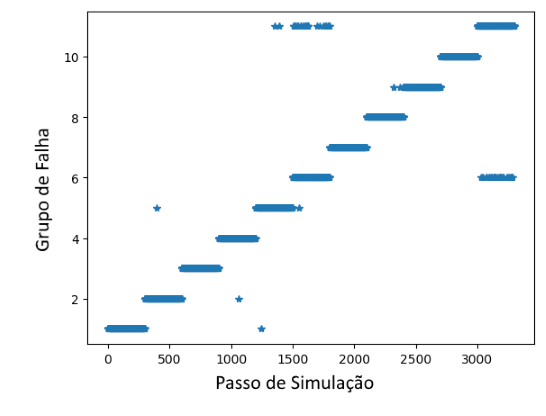
\includegraphics[width=13cm]{./01_Pre_textuais/nonlin_figs/RandomForestClassifier_Nonlinear_Rectfier_+_4bit_PRBS_[FALHA]_-_300_-_02sraw.png}
        \caption{\label{fig:randomforestClassifieRet}- Circuito: Retificador - Comportamento da Predição Random Forest }
        \end{center}
        \end{figure}

A percentual de acerto total é de 99,27\% para o circuito Retificador exemplificado na \ref{fig:randomforestClassifieRet} e \ref{tab:Retnrandom}. 

\newpage
 \item Classificador Gaussiano de Naive Bayes
 
 \begin{table}[ht]
\centering
\begin{tabular}{ccc}
\textbf{Classe} & \textbf{Acerto (\%)} & \textbf{Acurácia (\%)} \\
Classe 1        & 99,9                  & 99,9                    \\
Classe 2        & 99,9                  & 99,2                    \\
Classe 3        & 100                  & 100                    \\
Classe 4        & 99,8                  & 100                    \\
Classe 5        & 99,9                  & 99,7                    \\
Classe 6        & 98,2                  & 93,7                    \\
Classe 7        & 99,9                  & 100                    \\
Classe 8        & 99,9                  & 99,9                    \\
Classe 9        & 100                  & 99,9                    \\
Classe 10       & 100                  & 100                    \\
Classe 11       & 93,6                  & 97,3                                 
\end{tabular}
\caption{\label{tab:RetnGND}- Retificador: Falhas Gaussiano de Naive Bayes}
\end{table}


  \begin{figure}[H]
        \begin{center}
        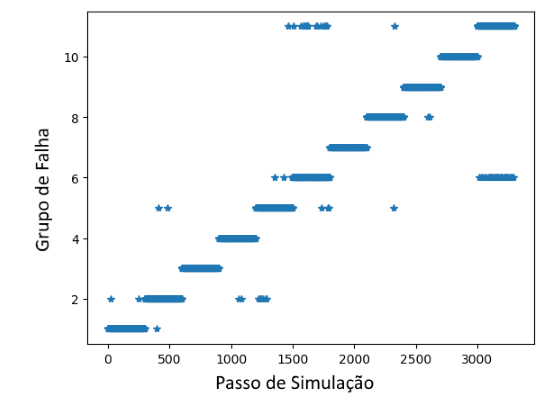
\includegraphics[width=13cm]{./01_Pre_textuais/nonlin_figs/GaussianNB_Nonlinear_Rectfier_+_4bit_PRBS_[FALHA]_-_300_-_02sraw.png}
        \caption{\label{fig:GaussianNBClassifieRet}- Circuito: Retificador - Comportamento Predição GaussianNB}
        \end{center}
        \end{figure}
		
A percentual de acerto total é de 99,19\% para o circuito Retificador exemplificado na \ref{fig:GaussianNBClassifieRet} e \ref{tab:RetnGND}. 
\newpage

 \item Classificador K vizinhos mais próximos
 
\begin{table}[ht]
\centering
\begin{tabular}{ccc}
\textbf{Classe} & \textbf{Acerto (\%)} & \textbf{Acurácia (\%)} \\
Classe 1        & 76,2                  & 68,7                    \\
Classe 2        & 78,2                  & 67                    \\
Classe 3        & 96,5                  & 100                    \\
Classe 4        & 85                  & 98,9                    \\
Classe 5        & 62,7                  & 93,2                    \\
Classe 6        & 76,9                  & 88,5                    \\
Classe 7        & 89,9                  & 100                    \\
Classe 8        & 95,6                  & 56,1                    \\
Classe 9        & 74,2                  & 99,7                    \\
Classe 10       & 99,3                  & 100                    \\
Classe 11       & 87,2                  & 64,3                                 
\end{tabular}
\caption{\label{tab:RetnKvizinhos}- Retificador: Falhas K vizinhos}
\end{table}


  \begin{figure}[H]
        \begin{center}
        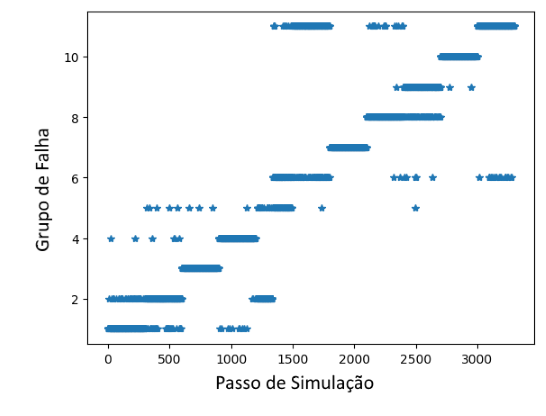
\includegraphics[width=13cm]{./01_Pre_textuais/nonlin_figs/KNeighborsClassifier_Nonlinear_Rectfier_+_4bit_PRBS_[FALHA]_-_300_-_02sraw.png}
        \caption{\label{fig:KNeighborsClassifieRet}- Circuito: Retificador - Comportamento da Predição K Neighbors }
        \end{center}
        \end{figure}

A percentual de acerto total é de 83,79\% para o circuito Retificador exemplificado na \ref{fig:KNeighborsClassifieRet} e \ref{tab:RetnKvizinhos}. 
\newpage

 \item Classificador Gradiente de descida estocástica
 
 \begin{table}[ht]
\centering
\begin{tabular}{ccc}
\textbf{Classe} & \textbf{Acerto (\%)} & \textbf{Acurácia (\%)} \\
Classe 1        & 99.9                  & 99.8                    \\
Classe 2        & 99.8                  & 100                    \\
Classe 3        & 100                  & 100                    \\
Classe 4        & 100                  & 100                    \\
Classe 5        & 100                  & 97,8                    \\
Classe 6        & 85,4                  & 92,3                    \\
Classe 7        & 97                  & 100                    \\
Classe 8        & 98,3                  & 98,4                    \\
Classe 9        & 97,5                  & 99,9                    \\
Classe 10       & 99                  & 100                    \\
Classe 11       & 87                  & 84                                   
\end{tabular}
\caption{\label{tab:RetnGDE}- Retificador: Falhas Gradiente de descida estocástica}
\end{table}

 \begin{figure}[H]
        \begin{center}
        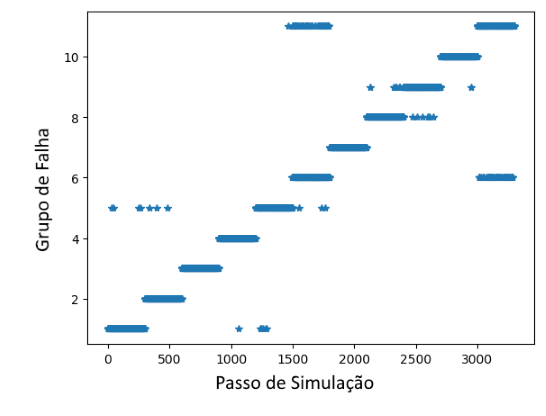
\includegraphics[width=13cm]{./01_Pre_textuais/nonlin_figs/SGDClassifier_Nonlinear_Rectfier_+_4bit_PRBS_[FALHA]_-_300_-_02sraw.png}
        \caption{\label{fig:SGDCClassifieRet}- Circuito: Retificador - Comportamento da Predição SGD}
        \end{center}
        \end{figure}
A percentual de acerto total é de 96,7\% para o circuito Retificador exemplificado na \ref{fig:SGDCClassifieRet} e \ref{tab:RetnGDE}. 

\newpage
 \item Classificador de Regressão logística 
 
 \begin{table}[ht]
\centering
\begin{tabular}{ccc}
\textbf{Classe} & \textbf{Acerto (\%)} & \textbf{Acurácia (\%)} \\
Classe 1        & 84,7                  & 99,7                    \\
Classe 2        & 91,3                  & 100                    \\
Classe 3        & 99,1                  & 100                    \\
Classe 4        & 99,6                  & 65,2                    \\
Classe 5        & 96,3                  & 76,4                    \\
Classe 6        & 81,2                  & 93.1                    \\
Classe 7        & 100                  & 100                    \\
Classe 8        & 91,3                  & 86                    \\
Classe 9        & 97,3                  & 98,2                    \\
Classe 10       & 99,5               & 99,7                    \\
Classe 11       & 97,3                  & 61                                 
\end{tabular}
\caption{\label{tab:Retnlogistic}- Retificador: Falhas Regressão logística}
\end{table}


  \begin{figure}[H]
        \begin{center}
        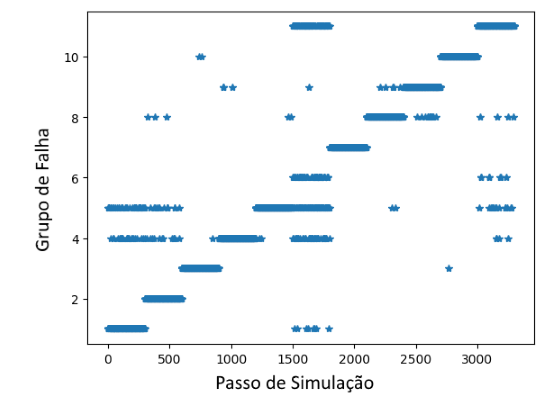
\includegraphics[width=12.5cm]{./01_Pre_textuais/nonlin_figs/LogisticRegression_Nonlinear_Rectfier_+_4bit_PRBS_[FALHA]_-_300_-_02sraw.png}
        \caption{\label{fig:LogisticRegressionClassifieRet}- Circuito: Retificador - Comportamento da Predição regressão Logística }
        \end{center}
        \end{figure}

A percentual de acerto total é de 94,32\% para o circuito Retificador exemplificado na \ref{fig:LogisticRegressionClassifieRet} e \ref{tab:Retnlogistic}. 
\end{itemize} 



\label{chapter:exemplo}

\section{\textbf{Resultados}}
Com todos os circuitos simulados, limpos, processados e com sua predição realizada, é possível analisar e comparar os melhores resultados. 

O resultado da predição foi verificado, e então calculado o percentual de acerto de cada um dos algoritmos para cada um dos circuitos. A quantidade percentual de acertos é exibida na \ref{tab:resultadoFinal}.

\begin{table}[H]
\centering
\begin{tabular}{cccccc}
\textbf{Algoritmo}     & \textbf{Circuito 1} & \textbf{Circuito 2} & \textbf{Circuito 3} & \textbf{Circuito 4} & \textbf{Média Acerto}           \\
\textbf{Arvore de D.}  & 9\%                 & 9\%                 & 5,2\%               & 9\%                 & 8,05\%                          \\
\textbf{AdaBoost}      & 99,96\%             & 80,72\%             & 66,3\%              & 99,57\%             & 86,63\% \\
\textbf{SVC}           & 12,06\%             & 25,33\%             & 20,36\%             & 27,27\%             & 21,25\%                         \\
\textbf{Floresta Ale.} & 100\%               & 77,55\%             & 66,63\%             & 99,27\%             & 85,86\%                         \\
\textbf{Naive Bayes}   & 99,87\%             & 81,87\%             & 66,39\%             & 99,19\%             & 86,83\% \\
\textbf{K vizinhos}    & 99,8\%              & 80\%                & 58,38\%             & 83,79\%             & 80,49\%                         \\
\textbf{GDE}           & 100\%               & 84,98\%             & 67,72\%             & 96,7\%              &86,8\%  \\
\textbf{Regressão L.}  & 99,96\%             & 78,53\%             & 53,02\%             & 94,32\%             & 60,20\%                        
\end{tabular}
\caption{\label{tab:resultadoFinal}- Comparação de desempenhos}
\end{table}


Através dos resultados exibidos na \ref{tab:resultadoFinal}, é possível verificar os algoritmos que melhor possuem o melhor desempenho nos diferentes tipos de circuitos. Devido a complexidade dos dados, os classificadores mais robustos obtiveram um melhor desempenho. O circuito 3 (CTSV), que possui uma maior quantidade de falhas e uma topologia mais elaborada, apresentou a maior dificuldade de ser classificado.

Os Algoritmos AdaBoost, Floresta Aleatória e o Gradiente de descida estocástica (GDE), apresentaram os melhores desempenhos sendo 86,63\%, 85,86\% e 86,83\% respectivamente. Importante destacar que alguns deles chegaram a atingir 100\% de acerto na classificação para alguns circuitos. 

Num passo a mais, foi testado a predição unindo os melhores resultados possíveis, ou seja, AdaBoost com estimador base de floresta aleatória. Esse conjunto apresentou uma taxa de acerto de quase 100\% para todos os circuitos.
